\documentclass{standalone}
\usepackage{tikz}
\begin{document}
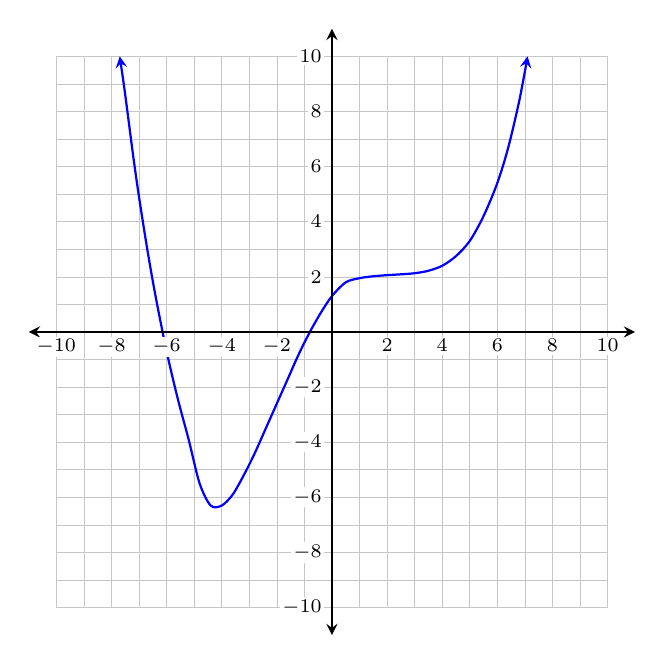
\begin{tikzpicture}[>=stealth, scale=0.35]
  % Same blank grid as 10B, with a sample answer graph drawn on it
  \draw[gray!45, very thin] (-10,-10) grid (10,10);
  % Quartic-shaped sketch: both ends rise, a single relative extremum
  % (the minimum near x = -4.2) and two points of inflection bounding
  % the flat stretch near y = 2
  \draw[<->, thick, blue] plot[smooth] coordinates
    {(-7.7,10) (-7.5,8.6) (-7.2,6.3) (-7.0,4.9) (-6.7,3.0) (-6.4,1.3)
     (-6.0,-0.7) (-5.6,-2.4) (-5.2,-3.9) (-4.8,-5.5) (-4.4,-6.3)
     (-4.0,-6.3) (-3.6,-5.9) (-3.2,-5.2) (-2.8,-4.4) (-2.4,-3.5)
     (-2.0,-2.6) (-1.6,-1.7) (-1.2,-0.8) (-0.8,0.0) (-0.4,0.7)
     (0,1.3) (0.5,1.8) (1.0,1.95) (1.5,2.02) (2.0,2.06) (2.5,2.09)
     (3.0,2.13) (3.5,2.22) (4.0,2.4) (4.5,2.75) (5.0,3.3) (5.5,4.2)
     (6.0,5.4) (6.4,6.7) (6.8,8.4) (7.1,10)};
  % Axes and labels drawn last so they sit on top of the curve
  \draw[<->, thick] (-11,0) -- (11,0);
  \draw[<->, thick] (0,-11) -- (0,11);
  \foreach \x in {-10,-8,-6,-4,-2,2,4,6,8,10} {
    \node[below, font=\scriptsize, fill=white, inner sep=1pt] at (\x,-0.15) {$\x$};
  }
  \foreach \y in {-10,-8,-6,-4,-2,2,4,6,8,10} {
    \node[left, font=\scriptsize, fill=white, inner sep=1pt] at (-0.25,\y) {$\y$};
  }
\end{tikzpicture}
\end{document}
